% Abbildung 2.1 -- Systemskizze des invertierten Pendels mit Winkelkonvention.
%
% Eigenstaendig kompilierbar (standalone-Klasse) zur Pruefung -- einfach mit
% pdflatex/Overleaf direkt uebersetzen, es entsteht eine zugeschnittene PDF.
%
% GEOMETRIE-CHECK gegen die Herleitung (protokoll.md §2.2 / Pendel_Herleitung_Ausfuehrlich.md §2):
%   x_p = s + l*sin(phi),  y_p = -l*cos(phi)   (Ursprung = Drehpunkt am Wagen)
%   phi = 0   -> (x_p,y_p) = (0,-l)  -> Masse haengt lotrecht nach unten
%   phi = 90  -> (x_p,y_p) = (l, 0)  -> Masse zeigt waagerecht nach rechts
%   phi = 180 -> (x_p,y_p) = (0, l)  -> Masse steht lotrecht nach oben (Ziel)
% Diese drei Stützstellen sind der schnellste Weg, die Zeichnung zu pruefen: unten,
% rechts, oben -- in genau dieser Reihenfolge, im Gegenuhrzeigersinn.
%
% In TikZ-Standardwinkeln (0 Grad = math. positive x-Achse, gegen den Uhrzeigersinn)
% entspricht das einer Verschiebung von 90 Grad: theta_tikz = phi_physik - 90 Grad.
% Der gezeichnete Pendel-Stab steht hier bei phi_physik = 50 Grad (ein generischer
% "Blickpunkt" zwischen phi=0 und phi=90, an dem der Winkel-Bogen gut lesbar ist),
% also theta_tikz = -40 Grad -- das ist der einzige "-40" unten im Code.
%
% Wenn's passt: entweder diese Datei zu PDF kompilieren und in report/images/ ablegen
% + per \includegraphics einbinden, ODER \usepackage{tikz} und
% \usetikzlibrary{calc,arrows.meta} in main.tex ergaenzen und den tikzpicture-Rumpf
% (zwischen \begin{tikzpicture} und \end{tikzpicture}) direkt in einer figure-Umgebung
% in chapters/02_grundlagen.tex per \input einbinden.

\documentclass[tikz,border=8pt]{standalone}
\usepackage[T1]{fontenc}
\usepackage{amsmath}
\usetikzlibrary{calc,arrows.meta}

\begin{document}
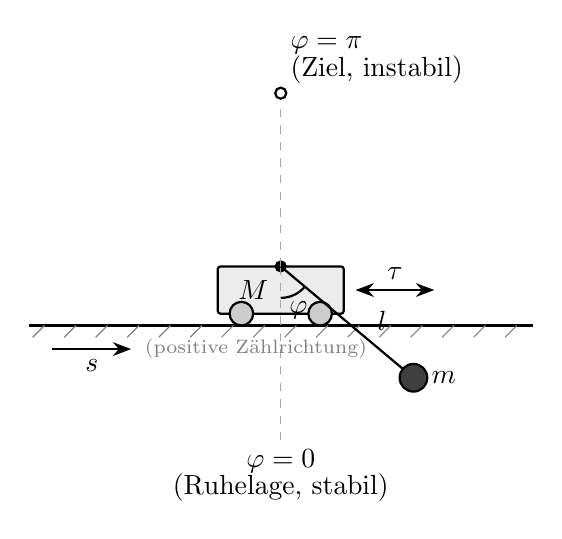
\begin{tikzpicture}[
  >=Stealth,
  cart/.style={draw, thick, fill=gray!15, rounded corners=1pt},
  wheel/.style={draw, thick, fill=gray!40},
  rod/.style={draw, thick},
  refline/.style={draw, dashed, gray!70},
  mass/.style={draw, thick, fill=black!75, circle},
]

% --- Schiene (mit Schraffur, rein dekorativ) ---
\draw[thick] (-3.2,0) -- (3.2,0);
\foreach \x in {-3.0,-2.6,...,3.0} {
  \draw[gray] (\x,0) -- ++(-0.15,-0.15);
}

% --- Wagen (Rechteck auf zwei Raedern) ---
\draw[cart] (-0.8,0.15) rectangle (0.8,0.75);
\draw[wheel] (-0.5,0.15) circle (0.15);
\draw[wheel] (0.5,0.15) circle (0.15);
\node at (-0.35,0.45) {$M$};

% --- Drehpunkt (Pivot) auf Wagenoberkante ---
\coordinate (pivot) at (0,0.75);
\filldraw[black] (pivot) circle (2pt);

% --- Referenzrichtungen: phi=0 (lotrecht unten) und phi=pi (lotrecht oben) ---
\draw[refline] (pivot) -- ++(0,-2.2) coordinate (down);
\draw[refline] (pivot) -- ++(0, 2.2) coordinate (up);
\filldraw[fill=white, draw=black, thick] (up) circle (2pt);

% --- Pendelstab in einer generischen Position phi_physik = 50 Grad ---
\coordinate (mass) at ($(pivot) + (-40:2.2)$);
\draw[rod] (pivot) -- (mass);
\filldraw[mass] (mass) circle (5pt);

% --- Winkel-Bogen von der phi=0-Referenz zur aktuellen Stabposition ---
\draw[thick] (pivot) ++(-90:0.4) arc (-90:-40:0.4);
\node at ($(pivot)+(-68:0.6)$) {$\varphi$};

% --- Beschriftungen der Referenzrichtungen ---
\node[below, align=center] at (down) {$\varphi = 0$\\[-2pt] (Ruhelage, stabil)};
\node[above right, align=left] at (up) {$\varphi = \pi$\\[-2pt] (Ziel, instabil)};

% --- Beschriftung von Stablaenge l und Pendelmasse m ---
\node at ($(pivot)!0.65!(mass) + (0.19,0.23)$) {$l$};
\node[right=3pt] at (mass) {$m$};

% --- Stellgroesse tau (Kraft auf den Wagen, bang-bang: +/-MAX_TAU per Pfeiltasten,
%     daher DOPPELT gerichteter Pfeil -- keine feste Fahrtrichtung) ---
\draw[<->, thick] (0.95,0.45) -- ++(1.0,0) node[midway, above] {$\tau$};

% --- Positionskoordinate s: nur die positive Zaehlrichtung der Koordinatenachse,
%     keine Aussage ueber die tatsaechliche Fahrtrichtung (die ist frei, s. tau oben) ---
\draw[->, thick] (-2.9,-0.3) -- ++(1.0,0) node[midway, below] {$s$};
\node[right, gray, font=\scriptsize] at (-1.85,-0.3) {(positive Zählrichtung)};

\end{tikzpicture}
\end{document}
